\documentclass[12pt,oneside,openany]{book} 
\setcounter{tocdepth}{3}
\usepackage{makeidx}           % allows index generation
\usepackage[dvips]{graphicx}          % standard LaTeX graphics to  when including figure files
\usepackage{multicol}          % used for the two-column index
\usepackage[dvips]{epsfig}
\usepackage{graphicx}
\usepackage{cite}
\usepackage{pifont}
\usepackage{amsmath}
\usepackage{amsfonts}
\usepackage{amssymb}
\usepackage{float}
\usepackage[spanish,es-noshorthands]{babel}
%\usepackage[toc]{appendix}
\usepackage[utf8]{inputenc}
\usepackage{booktabs}
\usepackage{fancyhdr}
\usepackage[subfigure,titles]{tocloft}
\usepackage{subfigure}         % for put subfigure
\usepackage{soul}
\usepackage{multirow}
\usepackage{centernot}
\usepackage{enumitem}
\usepackage{tikz}
\newcommand*\circled[1]{\tikz[baseline=(char.base)]{
		\node[shape=circle,draw,inner sep=2pt] (char) {#1};}}
\spanishdecimal{.}
\usepackage{multirow}
\usepackage{longtable}
\renewcommand\cftchapaftersnum{.}
\renewcommand\cftsecaftersnum{.}
\renewcommand\cftsubsecaftersnum{.}
\renewcommand\cftsubsubsecaftersnum{.}
\usepackage{verbatim}
\renewcommand\spanishtablename{Tabla}
\renewcommand\spanishbibname{Referencias}
\pagestyle{fancy}
\fancyhf{}
\rhead{Instituto Politécnico Nacional}
\lhead{Protocolo de tesis}
\rfoot{\thepage}

%\setlength{\oddsidemargin}{0.25in}
%\setlength{\evensidemargin}{0.1in}
%\setlength{\textwidth}{6.2in}
%\setlength{\topmargin}{0.0in}
%\setlength{\textheight}{9.1in}

\setlength{\oddsidemargin}{0.25in}
\setlength{\evensidemargin}{0.1in}
\setlength{\textwidth}{6.2in}
\setlength{\topmargin}{-0.3in}
\setlength{\textheight}{9in}

%%%%%%%%%%%%%%%%%%%%%%%%%%%%%%%%%%%%%%%%%%%%%%%%%%%%%

\newtheorem{propa}{Proposici\'{o}n}
\newtheorem{remarka}{Comentario}
\newtheorem{theorem}{Teorema}
\newtheorem{acknowledgement}[theorem]{Acknowledgement}
\newtheorem{algorithm}[theorem]{Algorithm}
\newtheorem{axiom}[theorem]{Axiom}
\newtheorem{case}[theorem]{Case}
\newtheorem{claim}[theorem]{Claim}
\newtheorem{conclusion}[theorem]{Conclusion}
\newtheorem{condition}[theorem]{Condition}
\newtheorem{conjecture}[theorem]{Conjecture}
\newtheorem{corollary}[theorem]{Corollary}
\newtheorem{criterion}[theorem]{Criterion}
\newtheorem{definition}[theorem]{Definition}
\newtheorem{example}[theorem]{Ejemplo}
\newtheorem{exercise}[theorem]{Exercise}
\newtheorem{lemma}[theorem]{Lemma}
\newtheorem{notation}[theorem]{Notation}
\newtheorem{problem}[theorem]{Problem}
\newtheorem{proposition}[theorem]{Proposición}
\newtheorem{remark}[theorem]{Comentario}
\newtheorem{solution}[theorem]{Solution}
\newtheorem{summary}[theorem]{Summary}
\newenvironment{proof}[1][Demostración]{\textbf{#1.} }{\ \rule{0.5em}{0.5em}}

%%%%%%%%%%%%%%%%%%%%%%%%%%%%%%%%%%%%%%%%%%%%%%%%%%%%%

\usepackage{graphicx}





\thispagestyle{empty}


\begin{document}
\begin{center}
	{\leftskip=-0.5in \mbox{ %\leftskip=-0.6in
			\begin{tabular}[c]{c}
				
				%\includegraphics[bb = 0 0 677 935,scale=0.102]{1_PORTADA/logoipn.jpg}
				
\includegraphics[scale=0.85]{figuras/IPN.eps}
				
			\end{tabular}
			
			\hspace{-0.1 in}%{-0.35 in}
			\begin{tabular}[c]{c}
				\Large \textbf{INSTITUTO POLIT\'ECNICO NACIONAL}\\ \\ \\
				\hspace{-0.1in} \large CENTRO DE INNOVACIÓN Y DESARROLLO\\ 
				\hspace{-0.1in} \large TECNOLÓGICO EN CÓMPUTO \\
			\end{tabular}
			\hspace*{-0.2in}
			\begin{tabular}[c]{c}
			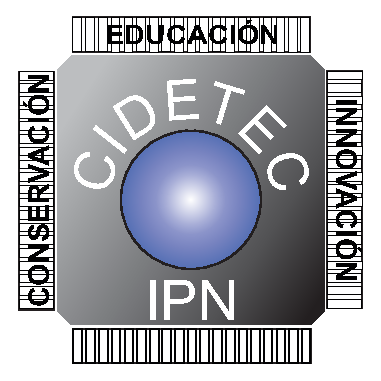
\includegraphics[scale=.4]{figuras/logo-cidetec.eps}
			\end{tabular}
		}
		\par
}	
	\vspace*{0.75in}

	\large{\textbf{DISEÑO E IMPLEMENTACIÓN DE ESQUEMAS DE CONTROL PARA CONVERTIDORES DE POTENCIA CD-CD}}\\
	
	
	
	\vspace*{0.65in}
	
	\makebox[0.55\textwidth][s]{\large \textbf{T E S I S}}\\
	\vspace*{0.2in}
	\makebox[0.55\textwidth][s]{\normalsize QUE PARA OBTENER EL GRADO DE:}\\
	\vspace*{0.2in}
	\large{\textbf{MAESTRÍA EN TECNOLOGÍA DE CÓMPUTO}}\\
	
	\vspace*{0.75in}
	
	\makebox[0.55\textwidth][s]{\normalsize P R E S E N T A:}\\ %
	\vspace*{0.15in}
	\makebox[0.61\textwidth]{\large \textbf{Ing. Adrián Jared Omaña Butrón}}\\
	
	\vspace*{0.75in}
	
	
	\centerline{\normalsize DIRECTORES DE TESIS:}
	\vspace*{0.125in}
	\scshape{
		Dr. Ramón Silva Ortigoza  \\
		Dra. Rosalba Galván Guerra\\
	}
	
	
	\vspace*{1in}
	
	\leftline{\large Ciudad de México, México} \vspace*{-0.25in} \rightline{\large
		Diciembre 2025}
	
	
\end{center}
\newpage
\tableofcontents
\thispagestyle{empty}
\newpage



\chapter{Introducción}

Los convertidores electrónicos de potencia son elementos presentes en diversos sistemas que requieren la transformación de energía eléctrica. Estas aplicaciones incluyen, entre otras, energías renovables, aeronáutica, vehículos eléctricos, robots y telecomunicaciones \cite{ref_journal1}. Estas aplicaciones requieren convertidores CD–CD capaces de mantener un voltaje de salida en un nivel deseado en un amplio rango de operación, aun en presencia de perturbaciones de carga, cambios en la fuente de entrada e incertidumbre de parámetros \cite{ref_journal2}, por lo cual resulta fundamental el desarrollo de técnicas de control que permitan satisfacer las necesidades energéticas de estos distintos tipos de aplicaciones.

Para estas aplicaciones, las topologías Buck, Boost y Buck–Boost representan bloques fundamentales debido a su capacidad para proporcionar niveles de voltaje menores, mayores o invertidos con respecto al voltaje de entrada. Sin embargo, la naturaleza conmutada de estos convertidores introduce dinámicas no lineales y sensibilidad ante perturbaciones, lo que dificulta garantizar una regulación precisa bajo condiciones de operación variadas.

En este contexto, el empleo de estrategias de control avanzadas se vuelve necesario para mejorar el desempeño dinámico, la robustez y la confiabilidad de estos sistemas. La presente tesis aborda el análisis, diseño y evaluación de técnicas de control aplicadas a estas topologías, con el fin de contribuir a su operación eficiente en escenarios reales.



\section{Estado del arte}


En esta sección se presentan los estudios más relevantes relacionadas a la implementación de controladores promedio, por modos dslizantes de primer orden y orden superior.

\subsection{Técnicas basadas en control promedio}

\subsection{Modo deslizante de primer orden} 

\subsection{Modo deslizante de orden superior}





\section{Planteamiento y justificaci\'on del problema}



Los convertidores de potencia CD–CD se encuentran presentes en una amplia gama de aplicaciones tecnológicas, tales como sistemas automotrices, aeronáuticos, embebidos, energéticos y microrredes. A pesar de su uso extendido y su importancia en la conversión eficiente de energía eléctrica, estos sistemas presentan no linealidades inherentes, así como alta sensibilidad ante perturbaciones en el voltaje de entrada y variaciones en la carga.

Los controladores diseñados mediante enfoques clásicos, particularmente aquellos basados en la linealización del modelo, pueden lograr una regulación aceptable bajo condiciones nominales. Sin embargo, su desempeño se ve comprometido cuando el convertidor opera ante perturbaciones significativas, cambios abruptos en la carga o exigencias dinámicas más estrictas. Esta limitación resulta especialmente crítica en aplicaciones donde se requiere robustez, alta estabilidad, rápida respuesta dinámica y seguimiento preciso de las variables de salida, como sucede en la alimentación de baterías, cargas electrónicas sensibles o cargas de potencia constante (CPL).

Debido a estas limitaciones, el estudio y desarrollo de esquemas de control no lineal para convertidores CD–CD resulta crucial. Estrategias como las basadas en control promedio, el control por modos deslizantes de primer orden (FOSM) y el control por modos deslizantes de orden superior (HOSM) ofrecen propiedades atractivas como robustez frente a incertidumbres, insensibilidad ante perturbaciones acotadas y regulación más precisa, lo que permite ampliar el rango operativo de los convertidores y garantizar un desempeño más confiable.

Las topologías buck, boost y buck-boost destacan por su amplia adopción en la industria, debido a que permiten generar un voltaje de salida menor, mayor o invertido respecto al voltaje de entrada. Cada una presenta desafíos propios asociados a su naturaleza no lineal y a las variaciones de carga. Por ello, el diseño, análisis y comparación de técnicas avanzadas de control aplicadas a estas tres topologías resultan esenciales para mejorar su desempeño, garantizar la estabilidad en múltiples condiciones de operación y facilitar su integración en aplicaciones modernas que demandan alta eficiencia energética, robustez y confiabilidad.

\section{Objetivos del trabajo}


A continuacion son presentados el objetivo general y objetivos particulares para la tematica a desarrollar.

\subsection{Objetivo general}

Desarrollar y evaluar esquemas de control basados en control promedio, modos deslizantes de primer orden (FOSM) y modos deslizantes de orden superior (HOSM) para los convertidores de potencia CD–CD Buck, Boost y Buck–Boost, orientados al seguimiento de una trayectoria de voltaje, verificados mediante simulación y experimentación.

\subsection{Objetivos particulares}

Los objetivos particulares que permitirán alcanzar el objetivo general son los siguientes:

\begin{enumerate}
	\item Obtener los modelos conmutados y promediados de los convertidores CD–CD Buck, Boost y Buck–Boost.
	
	\item Diseñar esquemas de control basados en control promedio, modos deslizantes de primer orden (FOSM) y modos deslizantes de orden superior (HOSM) para las tres topologías mencionadas.
	
	\item Implementar y simular los esquemas de control desarrollados utilizando el entorno MATLAB/Simulink y el toolbox Simscape Electrical.
	
	\item Realizar experimentos con los convertidores Buck, Boost y Buck–Boost, implementando los esquemas de control por modos deslizantes de primer orden y de orden superior.
	
	\item Validar el desempeño dinámico y la robustez de cada esquema de control mediante la comparación entre resultados simulados y experimentales.
	
	\item Documentar los resultados obtenidos durante el desarrollo de esta tesis.
\end{enumerate}

\section{Medios a emplear}
Los medios que se emplearán para alcanzar el objetivo de esta investigación son:

\begin{itemize}
\item Bases de datos científicas: Web of Science, Scopus y Google Académico.

\item Computadora de escritorio para la implementación del entorno de simulación y la interfaz con las tarjetas de adquisición de datos.

\item MATLAB–Simulink–Simscape Electrical 2025b para la modelación, simulación y evaluación de los esquemas de control.

\item Entorno de desarrollo integrado TeXStudio para la edición del documento en \LaTeX.

\item Conexión a internet para acceso a repositorios, bibliografía, herramientas de desarrollo y  control de versión.

\item Software para control de versiones: Git y GitHub.

\item Componentes electrónicos pasivos (resistencias, inductores, capacitores).

\item Fuentes de alimentación de corriente directa programables.

\item Tarjeta de adquisición de datos dSPACE DS1104.

\item Tarjeta de adquisición de datos dSPACE MicroLabBox.

\item Puntas de corriente Tektronix A622.

\item Puntas diferenciales de alta tensión Tektronix P5200A.
\end{itemize}

\section{Contenido del trabajo}
De manera preeliminar el presente trabajo estara conformado por los siguientes capitulos, Capitulo 1,
\newpage

\section{Cronograma de actividades}
En la Fig. \ref{fig1} se presenta el cronograma de actividades relacionado con esta propuesta de trabajo de tesis, con la finalidad de dar cumplimiento a los objetivos establecidos.

\begin{figure}[!ht]
	\centering
	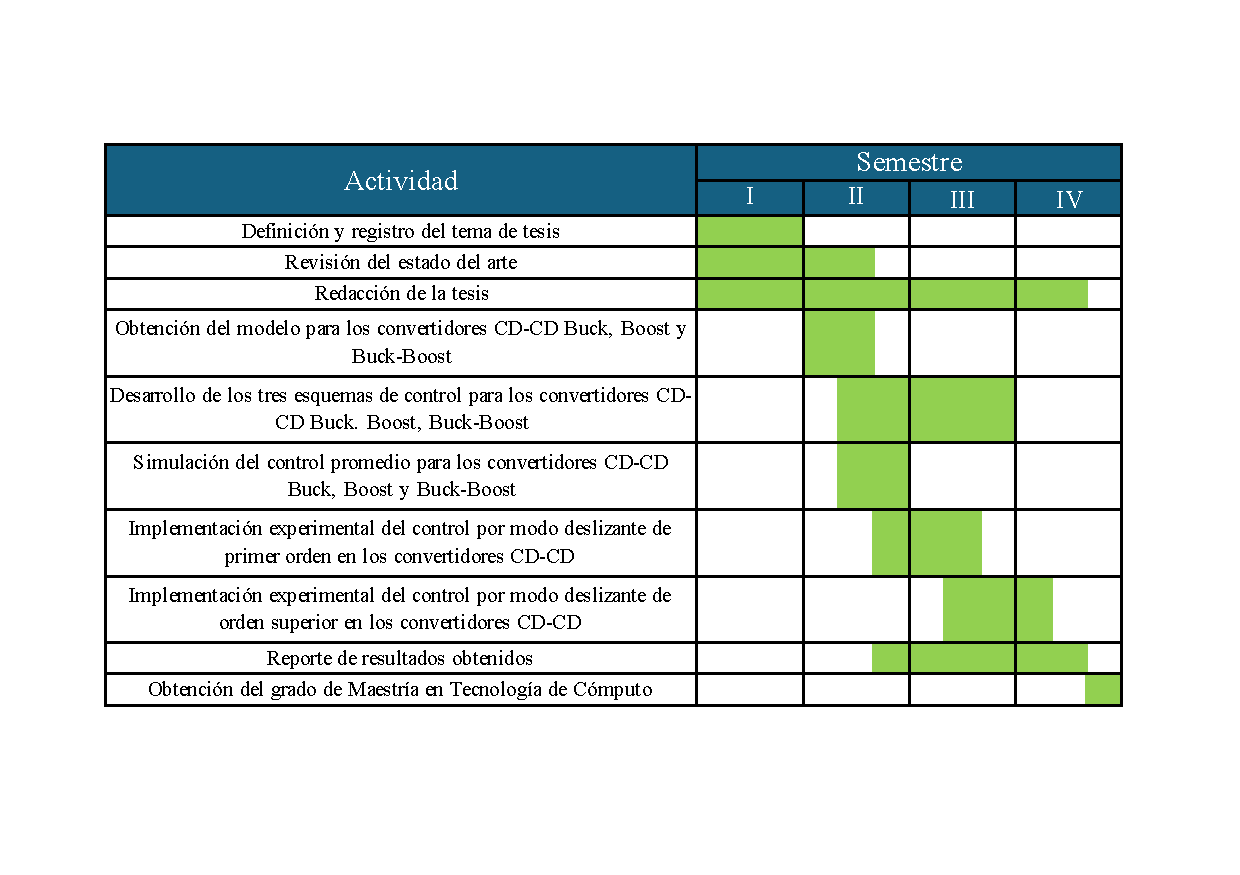
\includegraphics[scale=0.75]{figuras/Cronograma.pdf}
	\caption{Cronograma de actividades.}
	\label{fig1}
\end{figure}
1
\begin{thebibliography}{99}
\addcontentsline{toc}{chapter}{Referencias}	

%1
\bibitem{ref_journal1}
V. García-Rodríguez, R. Silva-Ortigoza, E. Hernández-Márquez, J. García-Sánchez, and H. Taud, “DC/DC Boost Converter–Inverter as Driver for a DC Motor: Modeling and Experimental Verification,”  \textit{Energies}, vol. 11, no. 8, p. 2044, Aug. 2018, doi: https://doi.org/10.3390/en11082044.
‌
\bibitem{ref_journal2}
S.-K. Kim, “Output Voltage-Tracking Controller With Performance Recovery Property for DC/DC Boost Converters,” \textit{IEEE Transactions on Control Systems Technology}, vol. 27, no. 3, pp. 1301–1307, May 2019, doi: https://doi.org/10.1109/tcst.2018.2806366.
‌




\end{thebibliography}

\end{document}